%----------------------------------------------------------------------------
\chapter{Background}\label{ch:background}
%----------------------------------------------------------------------------

In this chapter I address the foundations of this work. In \autoref{sec:formalisms} I introduce the theoretical bases of behaviour modeling, which is used widely in systems engineering, and their implementation in an existing language - SysML. After this I talk about Formal Verification in \autoref{sec:formal_verification}, which is a mathematically rigorous method for finding specific configurations of modelled systems. Lastly, I introduce the Gamma Composite Statechart Framework, which is a tool for stating and verifying composite models using statechart behaviours.

%----------------------------------------------------------------------------
\section{Modeling Formalisms}
%----------------------------------------------------------------------------

% TODO

Mondok Milán Bsc 2.2-höz hasonlóan: modellezési formalizmusok, activity formális leírása, petri net, tranzíciós rendszerek, stb
%----------------------------------------------------------------------------
\section{Formal Verification}\label{sec:formal_verification}
%----------------------------------------------------------------------------

Formal verification is a method for proving or disproving the correctness of a system with mathematical precision. Correctness is checked with respect to certain properties or specifications given by the user. Model checking is a formal verification technique that explores the behaviour of the given model exhaustively, i.e., all relevant behaviours of the model are analysed.

\begin{figure}[!ht]
	\centering
	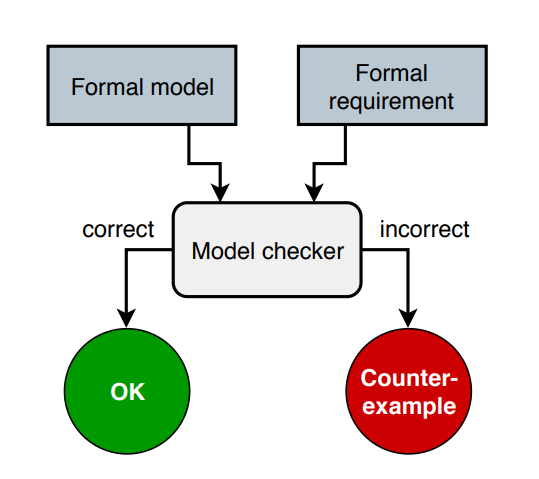
\includegraphics[width=67mm, keepaspectratio]{figures/model_checking.png}\hspace{1cm}
	\caption{An illustration of model checking.}
	\label{fig:model_checking}
\end{figure}

Formal verification tools require the formal model and a formal requirement as input, and return either an ok state, a counter example, or that it can't decide (see \autoref{fig:model_checking}). The counter example is the most important of all, as with its help, the engineers may have a chance of correcting the model.

%----------------------------------------------------------------------------
\section{The Gamma Statechart Composition Framework}\label{sec:gamma}
%----------------------------------------------------------------------------

The Gamma Statechart Composition Framework\footnote{https://inf.mit.bme.hu/en/gamma} \cite{mixed_statecharts_2020} is an integrated tool to support the design, verification and validation as well as code generation for component-based reactive systems. The behaviour of each component is captured by a statechart, while assembling the system from components is driven by a domain-specific composition language\footnote{The composition language be the \emph{ibd} model in SysML}. Gamma supports formal verification by mapping composite statecharts to a back-end model checker. Execution traces obtained as witnesses during verification are back-annotated as test cases to replay an error trace or to validate external code generators~\cite{molnar2018gamma}. 

\begin{figure}[!ht]
	\centering
	\includesvg[inkscapelatex=false, width=120mm, keepaspectratio]{gamma-functionality-overview}
	\caption{The overview of model transformation chains and modeling languages of the Gamma framework \cite{mixed_statecharts_2020}. The parts relevant to this work have been marked with red outline.}
	\label{fig:gamma-overview}
\end{figure}

The workflow of Gamma builds on a model transformation chain depicted in \autoref{fig:gamma-overview}, which illustrates the input and output models of these model transformations as well as the languages in which they are defined, and the relations between them. The modeling languages are as follows.

\begin{itemize}
	\item The \textbf{Gamma Statechart Language (GSL)} is a UML/SysML-based statechart language supporting different semantic variants of statecharts.
	\item The \textbf{Gamma Composition Language (GCL)} is a composition language for the formal hierarchical composition of state-based 	components according to multiple execution and interaction semantics.
	\item The \textbf{Gamma Genmodel Language (GGL)} is a configuration language for configuring model transformations.
	\item The \textbf{Gamma Property Language (GPL)} is a property language supporting the definition (CTL*) properties and thus, the formal specification of requirements regarding (composite)	component behavior.
	\item The \textbf{Gamma Trace Language (GTL)} is a high-level specification language for  execution traces of (composite) components.
\end{itemize}

Optionally, statechart models defined in supported modeling tools (front-ends) can be imported into Gamma (Step 1), which can be integrated according to well-defined execution and interaction semantics (Step 2). The resulting composite model is processed and transformed into the input formalisms of integrated model checker back-ends (Step 3). The model checker back-ends provide witnesses (diagnostic traces) based on specified properties, which are back-annotated, resulting in abstract traces (Step 4).
Finally, the abstract traces are mapped into concrete (executable) traces tailored to the targeted execution environment (Step 5). For a more detailed description, see \cite{mixed_statecharts_2020}.

\subsection{Example Statechart}

\autoref{lst:gamma-statechart} shows the Gamma Statechart representation of the State Machine introduced in \autoref{fig:sysml_state_machine}.

\begin{lstlisting}[float,language=statechart, caption={The traffic light controller state machine in the Gamma textual representation.}, label={lst:gamma-statechart}]
package TrafficLightCtrl
import "Interfaces"
statechart TrafficLightCtrl [
	port Control : requires Control
	port PoliceInterrupt : requires PoliceInterrupt
	port LightCommands : provides LightCommands
] {
	timeout BlinkingYellowTimeout3
	timeout BlackTimeout4
	transition from Yellow to Red when Control.toggle
	transition from Normal to Interrupted when PoliceInterrupt.police
	// ...
	transition from BlinkingYellow to Black when timeout BlinkingYellowTimeout3
	transition from Black to BlinkingYellow when timeout BlackTimeout4
	region main_region {
		state Normal {
			region normal {
				shallow history Entry2
				state Green {
					entry / raise LightCommands.displayGreen;
				}
				state Red {
					entry / raise LightCommands.displayRed;
				}
				state Yellow {
					entry / raise LightCommands.displayYellow;
				}
			}
		}
		state Interrupted {
			region interrupted {
				initial Entry1
				state Black {
					entry / set BlackTimeout4 := 500 ms; 
						raise LightCommands.displayNone;
				}
				state BlinkingYellow {
					entry / set BlinkingYellowTimeout3 := 500 ms; 
						raise LightCommands.displayYellow;
				}
			}
		}
		initial Entry0
	}
}
\end{lstlisting}
